\chapter{Implementation}
    \label{chap:implementation}

   This chapter will explain my implementation for this project. It will first give an overview of the architecture of the software product. After that, we will present each one of the challenges that have been implemented so far.

    \section{Architecture} 
        \label{sec:architecture}
        
    The central part of the software implementation consists of the Damn Vulnerable Mobile - Inter Component Communication app. This Android app contains all of the educational material needed to understand Android ICC and complete each challenge, encourages the user to learn interactively,  and it provides access to each challenge and to settings to control the challenge or the learning experience. 
    
    The rest of the project consists of a series of Android apps that play the role of either a vulnerable app or a malware. These apps are made to appear to be authentic apps with real-world functionalities, though many of them are nowhere close to full-feature app. Each challenge consists of an authentic scenario of a malware app attacking one of the vulnerable apps through one particular ICC vulnerability.
    
    The DVM-ICC app communicates with the challenge apps through the use of files in order to apply various settings to control the behaviour of the apps. These settings are explained in subsection \ref{subsec:challenge_settings}. Moreover, each pair of vulnerable and malicious apps communicate between each other as a result of the cyber attack, through the medium of Intents. The manner in which this communication takes place will be explained in detail for each challenge in section \ref{}.
    
    \section{DVM-ICC Application}
        \label{sec:home_app}
        
    In this section, I will explore the features of the DVM-ICC Android app. While doing so, I will explain the intended workflow that a user needs to follow and how app provides an educational experience. The follow description applies to the Beginner mode. The app has three different operation modes, which will be fully explained in subsection \ref{}.
    
    \subsection{Home Menu}
        \label{subsec:home_menu}
        
    \begin{wrapfigure}[18]{r}{0.4\textwidth}
        \centering
        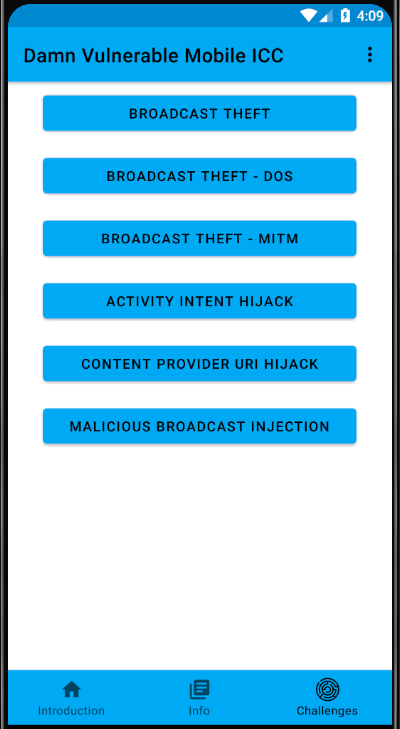
\includegraphics[width=0.4\textwidth]{graphics/home_activity.PNG}
        \caption{The first menu in the DVM-ICC app.}
        \label{fig:home_menu}
    \end{wrapfigure}
        
    The first screen the user sees when starting the app has 3 sub-pages: Introduction, Info and Challenges, as you can see in figure \ref{fig:home_menu}. The Introduction page gives an introduction of the project and explains the intended workflow for using the product. The Info page provides all of the necessary technical background to understand ICC vulnerabilities and attacks. It covers what components and permissions are, how components communicate between each other and the major types of ICC based attacks: Intent Hijacking and Intent Spoofing. The Challenges page lets the user select what challenge they want to start.
    
    \subsection{Challenge Settings}
        \label{subsec:challenge_settings}
        
    When clicking on a challenge, the user is taken to a menu where they can change the settings that define how the challenge will be undertaken. Here, you can set the operation mode for the challenge. Moreover, the user can enable or disable the malware of the selected challenge. If disabled, the malicious app will not perform any cyber-attack and therefore it will not interfere with any vulnerable app or the rest of the system.
    
    The most important settings on this screen is the security level of the vulnerable app. Inspired from DVWA, as described in subsection \ref{subsec:ICC_related_work}, these levels define how secure the vulnerable app is against attacks from the malware. Each challenge's vulnerable app has between 2 and 5 security levels, with each successive level using more secure code. This culminates with the Impossible level, where the vulnerability is fixed and the malware can not perform the attack. When the malware is enabled, it will overcome the defences of the current security level, except for the Impossible level. The number of security levels and their meaning depends on the challenge. In general, each security level means that a component or broadcast is protected with a more powerful permission, that components are no longer exported or that an intent is now sent explicitly. 
    
    The security level setting will dynamically change the code that the vulnerable app and malware of that challenge use, the user does not need to restart the apps, with some exceptions. The challenge settings can be changed at any time while doing a challenge.
    
    \subsection{Identifying the malware and the vulnerable app}
        \label{subsec:identify_challenge_apps}
        